\subsection{Išskirčių tyrimas}
Tyrėme HDI ir vaisinugmo rodiklio išskirtis.
Išskirtis tyrėme pasitelkdami kvartilių metodą. Tai reiškia, kad reikšmę laikėme sąlygine išskirtimi, jei ji priklausė intervalui $[Q1-3IQR; Q1-1,5IQR) \cup (Q3+1,5IQR; Q3+3IQR]$.

\begin{figure}[H]
    \centering
    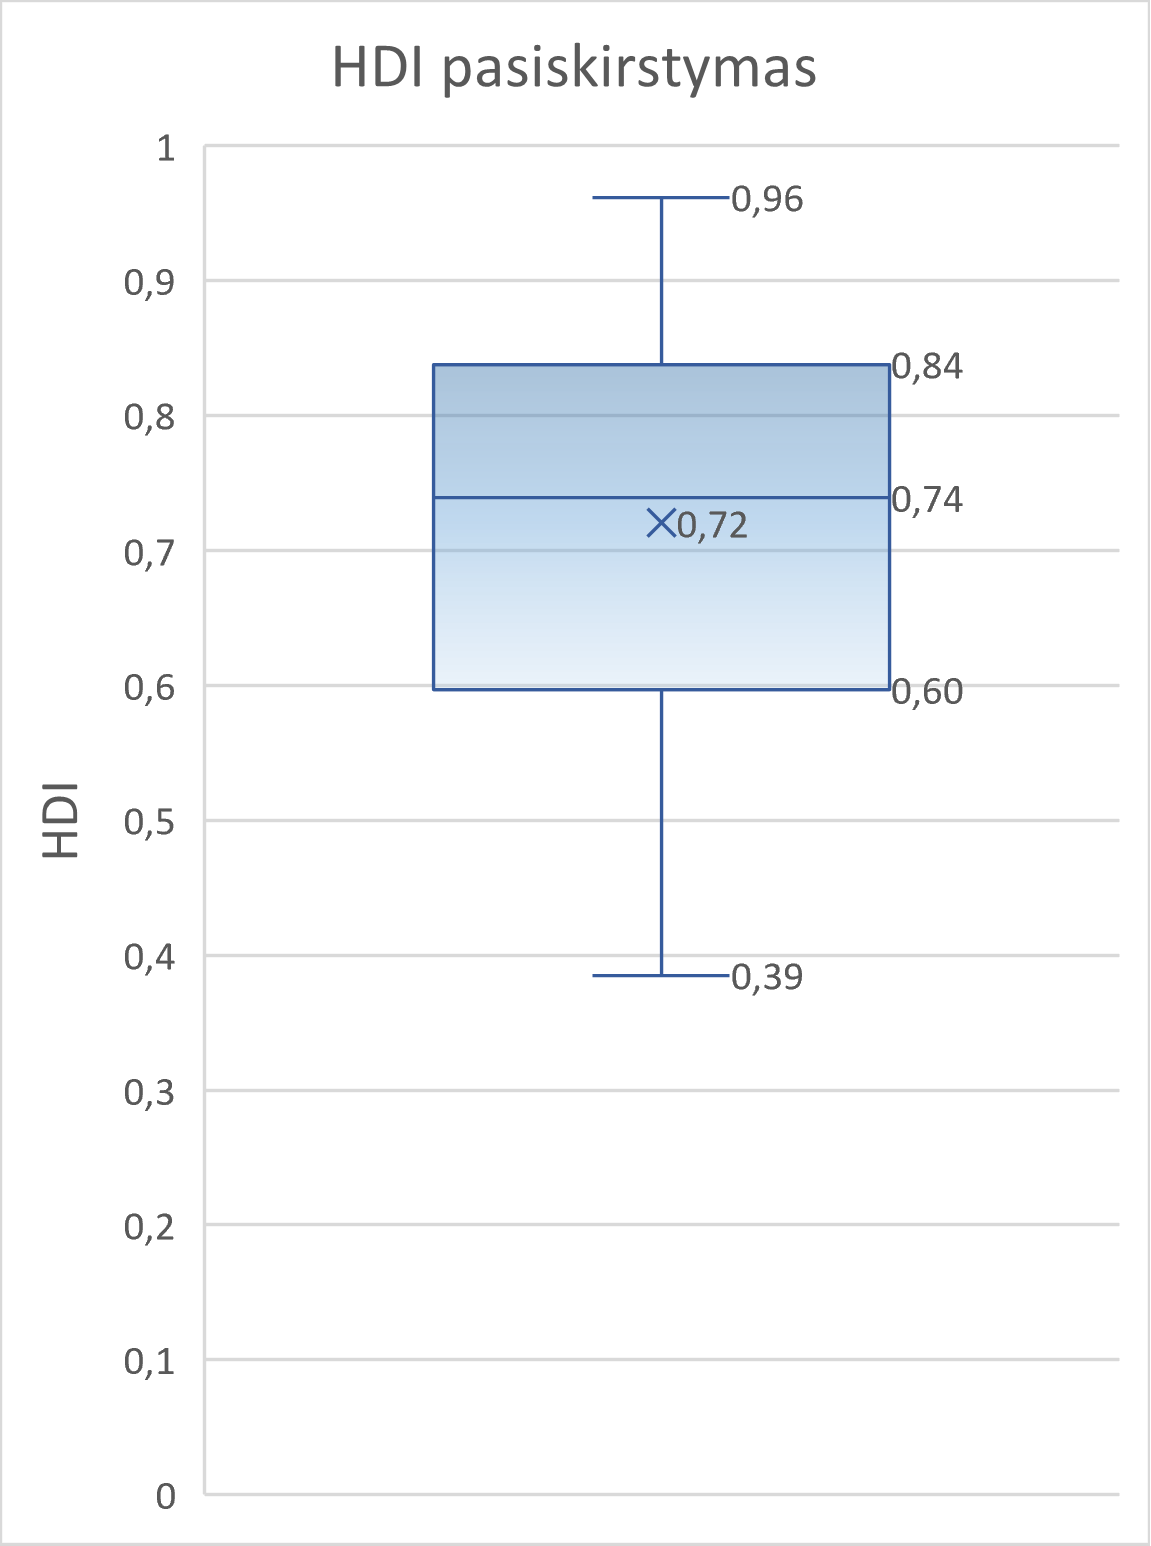
\includegraphics[width=.3\textwidth]{pic/box.png}
    \caption{HDI stačiakampė diagrama}
\end{figure}

\subsection{Koreliacijos tyrimas}
Pamatavome vaisingumo ir HDI bei vaisingumo ir aukštojo išsilavinimo procento rodiklių koreliacijas. Tai padarėme, pritaikydami Pirsono(angl. Pearson) koreliacijos koeficientą. Jis paskaičiuojamas pagal formulę: 
\begin{equation}
r = \frac{\sum\limits_i (x_i - \bar{x})(y_i - \bar{y})}{\sqrt{\sum\limits_i(x_i - \bar{x})^2}\sqrt{\sum\limits_i(y_i - \bar{y})^2}}
\end{equation}

Tyrimo rezultatus pateikiame lentelėje:
\begin{table}[H]
\begin{center}
    \begin{tabular}{|c|c|}
        \hline
        \textbf{Lyginti kintamieji} & \textbf{Pirsono koreliacijos koeficientas} \\\hline
        HDI ir Vaisinigumo rodiklis & -0,819 \\\hline
        Aukštojo išsilavinimo procentas ir vaisingumo rodiklis & -0,399 \\\hline
    \end{tabular}
    \caption{Koreliacijos skaičiavimų rezultatai}
\end{center}
\end{table}

Šių kintamų sąryšius iliustruoja sklaidos diagramos:
\begin{multicols}{2}
\diagrama{pic/vias_hdi_rod.png}{Gyventojų vaisingumo rodiklio ir HDI sklaidos diagrama}
\diagrama{pic/gyv_vais_kor.png}{Gyventojų vaisingumo rodiklio ir aukštojo išsilavinimo procento sklaidos diagrama}
\end{multicols}

\subsection{Aukštąjį išsilavinimą gavusiųjų suaugiusiųjų pasiskirtsymo tyrimas} 

Aukštąjį išsilavinimą gavusių suaugiusiųjų pasiskirtsymą iliustruoja histograma:
\diagrama{pic/histo.png}{Gyventojų vaisingumo rodiklio ir HDI sklaidos diagrama.}

\subsection{Vaisingumo pasiskirstymas pasaulyje}
Tirdami šį pasiskirstymą pagal šalis pastebime tendenciją:
\diagrama{pic/map.png}{Vaisingumo rodiklis įvairiose pasaulio šalyse.}

Tirdami šį pasiskirstymą pagal žemynus nupiešiame skritulinę diagramą:
\diagrama{pic/pie_2020.png}{Skritulinė diagrama, vaizduojanti vaisingumą įvairiuose žemynuose}

\subsection{Vaisingumo rodiklis Baltijos šalyse}
Mums buvo svarbu nustatyti, kaip skiriasi minėti rodikliai tarp Baltijos šalių.
Tam mums pravertė stulpelinė diagrama:
\diagrama{pic/balt.png}{Įvairūs rodikliai Baltijos šalyse}

Taip pat, mes tyrėme, kaip keitėsi Baltijos šalių vaisingumo rodiklis tarp 1960 ir 2021 metų.
\diagrama{pic/vais_balt.png}{Baltijos šalių vaisingumo rodiklis įvairiais metais}
